\documentclass[12pt,a4paper]{article}
\usepackage{times}
\usepackage{durhampaper}
\usepackage{url}
\usepackage{amsmath}
\usepackage{harvard}
\usepackage[utf8x]{inputenc}
\usepackage{wrapfig}
\usepackage{booktabs}
\usepackage{graphicx}

\usepackage{titlesec}
\setcounter{secnumdepth}{4}
\usepackage{cite}
\citationmode{abbr}
\bibliographystyle{plain}
\renewcommand*{\arraystretch}{0}

\title{An Analysis of Machine Learning and Deep Learning Techniques for Detecting Sarcasm in Online Text}
\author{} % leave; your name goes into \student{}
\student{Molly Hayward}
\supervisor{Dr Noura Al-Moubayed}
\degree{BSc Computer Science}

\date{}

\begin{document}

\maketitle

\begin{abstract}
\\ \indent \textbf{Context / Background --} 
Sarcasm is a unique form of language that cannot be interpreted at surface-level. Detecting sarcasm proves a significant challenge for traditional sentiment analysers and humans alike. This highlights the scope for innovative machine learning and deep learning solutions to this ill-structured problem.

\indent \textbf{Aims --} Despite the challenges in this domain, the ultimate aim of this project was to produce a tool that can be used to detect sarcasm with a \textit{high degree} of accuracy. 

\indent \textbf{Method --} In my endeavour to realise this aim, I used state-of-the-art contextualised word embeddings and deep learning classification models.

\indent \textbf{Results --} Through extensive experimentation, I found that

\indent \textbf{Conclusions --} Following this experimentation, I conclude that

This section should not be longer than half of a page, and having no more than one or two sentences under each heading is advised. Do not cite references in the abstract.
\end{abstract}

\begin{keywords}
Machine learning, Deep learning, Sarcasm Detection, Sentiment Analysis, Classification
\end{keywords}


\section{Introduction}
\noindent Sarcasm is a complex linguistic phenomenon, which when present in text indicates that the literal interpretation differs from the implied meaning. Sarcasm is prevalent in online user-generated content, and poses a significant challenge within the field of natural language processing, specifically within sentiment analysis, as it inverts the sentiment-polarity of a positive or negative utterance. Sentiment analysis is the task of deducing the sentiment polarity of text - typically whether the author is in favour of, or against, a certain subject. It is increasingly common for organisations to use sentiment analysis in order to gauge public opinion on their products and services; however, classic sentiment analysers cannot deduce the implicit meaning of sarcastic text and will wrongly classify the author's opinion. Hence, any tool that strives to accurately determine the meaning of user-generated text must be capable of detecting sarcasm. The phenonmenon of sentiment incongruity often lies at the heart of sarcasm, therefore advancements in automatic sarcasm detection research have the potential to vastly improve the sentiment analysis task.

\subsection{Problem Background}
\noindent As sarcasm is multi-faceted, this makes its detection a unique and interesting challenge. It can be both explicit and implicit; oftentimes, contextual cues are more powerful indicators of sarcasm than the words themselves. However we often lose this context, and hence the sarcastic undertones, in transcription. Consider the scenario where a person is congratulated on their hard work, despite the obviousness of them having not worked hard at all. Or perhaps a customer thanking a waiter for the delicious food, even though they sent it back to the kitchen. In isolation, the speech is not enough to convey the sarcastic intent. Furthermore, even humans struggle to consistently recognise sarcastic intent; due in part to the lack of an all-encompassing, universal definition of sarcasm. In a 2011 study, Gonz{\'a}lez-Ib{\'a}nez et al. \cite{gonzalez2011identifying} found low agreement rates between human annotators when classifying statements as either sarcastic or non-sarcastic, and in their second study, three annotators unanimously agreed on a label less than 72\% of the time. Truly, the existence of sarcasm can only be conclusively affirmed by the author. Additionally, developmental differences such as autism, as well as cultural and societal nuances cause variations in the way different people define and perceive sarcasm.

These factors make sarcasm detection an extremely complex task for both humans and computers. Despite this, \textit{most} humans can recognise sarcastic intent \textit{most} of the time. If we could replicate this performance, or even perhaps improve upon it, we could move towards a more concrete definition of what \textit{makes} a statement sarcastic. This highlights the scope for automating this process, and the need for an innovative solution.

\subsection{Research Questions and Objectives}
\noindent The \textbf{research questions} guiding this project are as follows --
\\ \indent \textit{Which linguistic cues indicate sarcastic intent in written text? How can a model be used to detect the words that correlate more to sarcastic labels? Do deep learning techniques perform better than machine learning approaches for sarcasm detection? Can the solution be used to improve the sentiment analysis task? Does the proposed solution perform well on other datasets?}\\

\noindent The following objectives were designed to address these specific research questions, and have been divided into three categories depending on their priority level and difficulty.

The \textbf{minimum} objectives of this project were to evaluate, compare and clean high-quality datasets, as well as to experiment with and evaluate machine learning architectures on these datasets. I achieved this by ...

The \textbf{intermediate} objectives of this project were to experiment with and evaluate deep learning models on the chosen datasets, and determine which is the best performing solution. Additionally, I also evaluated the model against unseen data. I achieved this by...

The \textbf{advanced} objectives of this project were to implement an attention-based deep neural network in order to identify words that correlate more to sarcastic labels, in order to produce a visualisation of attention words. I achieved this by ...




%This section briefly introduces the general project background, the research question you are addressing, and the project objectives.  It should be between 2 to 3 pages in length.\\%

\vfill

\section{Related Work}
\noindent In this section, we will compare classification model architectures used specifically in sarcasm detection research, as well as techniques that have seen success in other natural language processing (NLP) classification tasks as they may have potential to perform well in this specific domain. In most approaches, sarcasm detection is treated as a binary classification problem, in which text is grouped into two categories - sarcastic and non-sarcastic. It is otherwise treated as a multi-class problem where the extent to which a statement is sarcastic is ranked on a discrete scale, e.g. 1 to 5. 
In similar studies, the terms irony and sarcasm are often used interchangeably \cite{tsur2010icwsm}. For clarity, an overview of their definitions are given in figure 1. Both definitions capture the humourous intent in both sarcasm and irony, however sarcasm extends this definition to include the potential for criticism - often present in opinion-based content such as product reviews.

\begin{center}
	\textbf{Figure 1}: Comparison of defintions of Irony and Sarcasm
\end{center}
\begin{center}
\begin{tabular}{p{2cm}p{12cm}}
	\hline\vspace{0.5pt}
	\textbf{Term} & \vspace{0.5pt}\textbf{Definition}\\[1.2ex]
	\hline\hline
	Irony & The use of words that are the opposite of what you mean, as a way of being funny. \cite{cambridgeirony2020}\\
	\hline
	Sarcasm & The use of remarks that clearly mean the opposite of what they say, made in order to hurt someone's feelings or to criticize something in a humorous way. \cite{cambridgesarcasm2020}\\
	\hline
\end{tabular}\\
\end{center}

\subsection{Traditional Classifiers}
\noindent A number of simple linguistic approaches have been used in previous research. One such class of na\"{i}ve approaches is \textit{rule-based}, where text is classified based on a set of linguistic rules. Maynard and Greenwood (2014) \cite{maynard2014cares} proposed that the sentiment contained in hashtags can indicate the prescence of sarcasm in tweets, such as \#notreally in the example "I love doing the washing-up \#notreally". They used a rule-based approach, whereby if the sentiment of a tweet contradicts that of the hashtag, then this tweet is labelled sarcastic. They reported an $F_{1}$ score of 91.03\% on a random sample consisting of 400 tweets.

In Riloff et al. (2013) \cite{riloff2013sarcasm}, sarcasm is described as a contrast between positive sentiment and negative situation. This description is leveraged by Bharti et al (2015) \cite{bharti2015parsing}, which presents two rule-based approaches to sarcasm detection. The first approach identifies sentiment bearing situation phrases, classifying the phrase as sarcastic if the negative situation is juxtaposed with a positive sentiment phrase. Rule-based techniques are fairly primitive when compared to their modern, deep learning counterparts, as each ruleset must be generated manually and for each dataset.

\subsection{Machine-Learning Classifiers}
\noindent Using both labelled and unlabelled training data, a machine-learning algorithm can learn patterns that are associated with each category of data. This allows it to classify unseen text into these categories without the need for a static linguistic rule set. If the training data is high-quality and plentiful, the model can begin to make accurate predictions. There are a few general architectures of machine-learning classifiers, including Na\"{i}ve Bayes, Support Vector machines (SVMs) and logistic regression based classifiers. Although, not all approaches fit neatly into these categories.

Tsur et al. (2010) \cite{tsur2010icwsm} proposed a novel semi-supervised algorithm, \textit{SASI}, for sarcasm identification; trained on a small balanced seed of 160 reviews (80 sarcastic and 80 non-sarcastic) from a corpus of 66000 human-annotated Amazon product reviews. In order to mimic the ambiguous and spectral nature of sarcasm, a discrete score between 1 (non-sarcastic) and 5 (definitely sarcastic) is assigned to each sentence; scores of 3 and higher indicate sarcasm. Syntactic and pattern-based features are extracted and fed to a classifier which utilizes a strategy similar to k-nearest neighbor (kNN), whereby a sarcasm score is assigned to an unseen vector based upon the weighted average of the k-nearest neighbors in the training set. They reorted an $F_{1}$ score of 82.7\% on the binary classification task

Na\"{i}ve Bayes classifiers are supervised algorithms that use bayes theorem to make predictions. Reyes et al. (2013) \cite{reyes2013multidimensional} used a na\"{i}ve bayes and decision trees algorithm in order to detect irony which is closely related to sarcasm. They experimented with balanced and unbalanced distributions (25\% ironic tweets and 75\% other), achieving an F-score of 0.72 on the balanced distribution, dropping to 0.53 for the inbalanced distribution. In a similar vein, Barbieri et al. (2014) \cite{barbieri2014modelling} used random forest and decision tree classifiers, also for the detection of irony. They used six types of features in order to represent tweets, and recorded results over three categories of training data - education, humor and politics.

Support Vector Machines (SVM), can be effective when smaller amounts of training data are available, however they require more computational resources than na\"{i}ve bayes. SVMs use kernel functions to draw hyperplanes dividing a space into subspaces. Gonz{\'a}lez-Ib{\'a}nez et al\. (2011) \cite{gonzalez2011identifying} used two classifiers, support vector machine with sequential minimal optimization, as well as logistic regression. Their best result was an accuracy of 0.65, achieved with the combination of support vector machine with sequential miniminal optimization and unigrams. \textit{Pt{\'a}{\v{c}ek et al. (2014)}} \cite{ptavcek2014sarcasm} also used support vector machine and Maximum Entropy classifiers. They also performed classification on balanced and inbalanced distributions.

\subsection{Deep-Learning Classifiers}
Deep neural networks (DNNs) are increasingly being used in text classification tasks \cite{zhang2015character, poria2016deeper}. Two common DNN architectures are Recurrent Neural Networks (RNNs) and Convolutional Neural Networks (CNNs). They typically require a lot more training data than machine learning algorithms, but have been shown to produce state-of-the-art results in several domains.

https://arxiv.org/pdf/1703.03091.pdf

This has already been used
Write about RNN uses

One particularly interesting technique is the \textit{Hierarchical Attention Network (HAN)} defined in Yang et al. (2016) \cite{yang2016hierarchical} - an attention-based LSTM. The intuition is that certain words and sentences in a document contribute more to its overall meaning, and this is highly context dependent. They included one attention mechanism at word-level and another at sentence-level, and this allowed them to determine which words and phrases correlate more to certain labels. Using a similar approach in the domain of sarcasm may allow me to highlight the attention-words that are strongly influence the level of sarcasm. A similar technique was applied in \textit{Ghosh et al. 2018)} \cite{ghosh2018sarcasm} where they concluded that emoticons such as ':)' and interjections e.g. "ah", "hmm" correspond with highly weighted sentences. 
Gated Recurrent Units (GRUs) are another type of RNN used to overcome the vanishing gradient problem.  \textit{Zhang et al. (2016)} \cite{zhang2016tweet} used a bidirectional gated RNN to capture local information in tweets, as well as a pooling neural network to extract context from historic tweets, achieving 78.55\% accuracy.

Convolutional Neural Networks allow us to extract higher-level features, and they are based on the mathematical operation of convolution. \textit{Zhang et al. (2015)}  \cite{zhang2015character} explored the used of character-level convolutional neural networks for text classification. This network consists of 6 convolutional layers and 3 fully-connected layers. They found that it showed better peformance on raw texts such as an Amazon product review corpus. CNNs have been previously used in sarcasm detection. For example, \textit{Poria et al. (2017)} \cite{poria2016deeper} describes a convolutional neural network (CNN) for sarcasm detection. \\


%This section presents a survey of existing work on the problems that this project addresses.  it should be between 2 to 4 pages in length.  The rest of this section shows the formats of subsections as well as some general formatting information for tables, figures, references and equations. Note that the whole report, including the references, should not be longer than 20 pages in length.  The system will not accept any report longer than 20 pages.  It should be noted that not all the details of the work carried out in the project can be represented in 20 pages.  It is therefore vital that the Project Log book be kept up to date as this will be used as supplementary material when the project paper is marked.  There should be between 10 and 20 referenced papers---references to Web based pages should be less than 10\%.





%The font used for the main text should be Times New Roman (Times) and the font size should be 12.  The first line of all paragraphs should be indented by 0.25in, except for the first paragraph of each section, subsection, subsubsection etc. (the paragraph immediately after the header) where no indentation is needed.


%In general, figures and tables should not appear before they are cited.  Place figure captions below the figures; place table titles above the tables.  If your figure has two parts, for example, include the labels ``(a)'' and ``(b)'' as part of the artwork.  Please verify that figures and tables you mention in the text actually exist.  make sure that all tables and figures are numbered as shown in Table \ref{units} and Figure 1.
%sort out your own preferred means of inserting figures


%The list of cited references should appear at the end of the report, ordered alphabetically by the surnames of the first authors.  References cited in the main text should use Harvard (author, date) format.  When citing a section in a book, please give the relevant page numbers, as in \cite[p293]{budgen}.  When citing, where there are either one or two authors, use the names, but if there are more than two, give the first one and use ``et al.'' as in  , except where this would be ambiguous, in which case use all author names.


%You need to give all authors' names in each reference.  Do not use ``et al.'' unless there are more than five authors.  Papers that have not been published should be cited as ``unpublished'' \cite{euther}.  Papers that have been submitted or accepted for publication should be cited as ``submitted for publication'' as in \cite{futher} .  You can also cite using just the year when the author's name appears in the text, as in ``but according to Futher \citeyear{futher}, we \dots''.  Where an authors has more than one publication in a year, add `a', `b' etc. after the year.

\section{Solution}
\noindent This project addresses a binary classification problem, aiming to identify if a given snippet of text is sarcastic or non-sarcastic. First, the data is collected and pre-processed. Then, features are extracted and the data is vectorised. These vectors are used to train to a classifier, which is then carefully evaluated in order to account for potential overfitting. The following figure outlines the model pipeline, and each of these stages are further addressed in the remaining sections.

\begin{center}
	\textbf{Figure 2:} Overview of the model pipeline
\end{center}
\begin{center}
	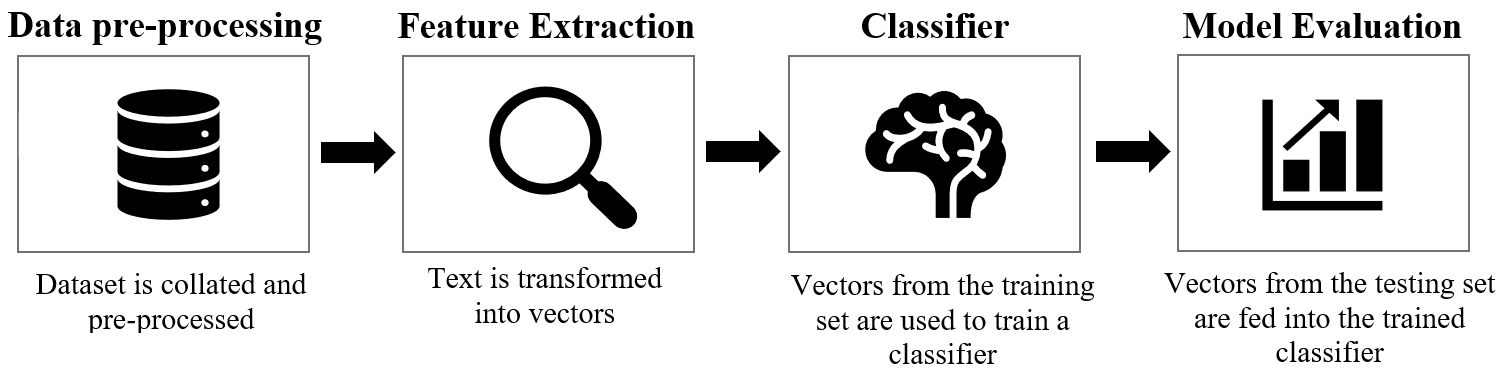
\includegraphics[width=0.8\textwidth]{Images/modelpipeline2.png}
	\label{Model Pipeline}
\end{center}

\subsection{Implementation Tools}
\noindent This project was majoritively written in \textbf{Python}, as it has an abundance of open-source libraries well-suited to machine learning and deep-learning tasks. Additionally, Python is very readable, making it easy for others to interpret, test and reproduce code. We used \textbf{pandas} for manipulating the datasets, as it provides functionality for applying functions globally across the dataset. We used \textbf{pickle} to store the vectorised datasets in memory. Vectorisation is a costly process, therefore writing the files to memory reduces long-term time demands during the experimentation and testing phases. We also  incorporated \textbf{SpaCy} when cleaning and tokenizing the data.

In terms of \textit{classification}, we did most of the machine learning implementation using \textbf{scikit-learn} - an open-source machine learning library. For constructing deep learning models, we used \textbf{keras}, as its modular structure allows for extensive experimentation and facilitates simple tweaking of model architectures. The model interface was written using web-application development languages such as HTML, CSS and JavaScript.

\subsection{Datasets}
\noindent In similar studies, large datasets have been collected, and in some cases, made publically available. We evaluated the suitability of many of these datasets and selected four which were used in this project. We experimented with data from multiple domains and online platforms, including Twitter, Amazon, Reddit and News outlets. This gives a broad coverage of the way sarcasm is used under different circumstances and in both formal and informal media. We evaluated many datasets and evaluated their suitability based on statistics from the dataset and desired attributes. For example, we avoided using datasets containing tweet ids, whereby the original tweet must be scraped using the Twitter API. We found that a small portion of the original tweets are no longer available on twitter, therefore this would not make for a fair comparison between my results and the results of the source study.

Four datasets were selected, and a statistical break down of their properties is provided in figure 3, including the number of instances in the dataset, the average number of tokens in each instance and the percentage of tokens that are included in the GloVe dictionary. GloVe is a method of feature extraction where word embeddings for tokens are provided as a dictionary. The number of tokens present in the GloVe dictionary is a measure of quality, as this method of feature extraction cannot be used on instances that contain many ill-formed and unrepresented tokens. Additionally, all tokens were converted to lowercase beforehand to make for a fair comparison between datasets, as only lowercase tokens are present in the GloVe dictionary. A detailed explanation of GloVe is provided in the feature extraction section.

\begin{center}
	\textbf{Figure 3}:  Statistical breakdown of the datasets used in this project
\end{center}
\begin{center}
	\begin{tabular}{p{4.3cm}p{2.1cm}p{2.6cm}p{2.2cm}p{1.8cm}}
		\toprule
		\textbf{Dataset Title} & \textbf{Number of data points} & \textbf{Avg. \#tokens} & \textbf{\% in GloVe dictionary} & \textbf{Benchmark}\\
		\midrule\midrule
		News Headlines Dataset For Sarcasm Detection & \begin{tabular}{c@{}@{}@{}} \\28619\\[1ex] +ve: 47.6\% \\[1ex] -ve: 52.4\% \end{tabular} &  11.2 tokens & 97.8\% & 89.7\%\\[1ex]
		\midrule
		Sarcasm Amazon Review Corpus & \begin{tabular}{c@{}@{}@{}} \\1254\\[1ex] +ve: 34.9\% \\[1ex] -ve: 65.1\% \end{tabular} &  276.4 tokens & 98.2\% & j \\[1ex]
		\hline
	\end{tabular}\\
\end{center}
\vspace{2pt}

\begin{enumerate}
	\item \textbf{News Headlines Dataset For Sarcasm Detection} -- \textit{Misra et al. (2019)} \cite{misra2019sarcasm}\\ Headlines are collected from two news sources - \textit{The Onion} \cite{onion2020} and \textit{The Huffington Post} \cite{huffpost2020}. The Onion is renowned for posting satiricial news, and these sarcastic headlines account for the sarcastic instances in the dataset. The non-sarcastic instances were collected from the Huffington Post. There is little noise in this dataset, as news headlines are written formally, and are far less likely to contain spelling and grammar errors than data from more informal platforms. These headlines are self contained, unlike tweets which may be in response to another tweet, thereby excluding necessary context. Misra et al. (2019) \cite{misra2019sarcasm} used a hybrid neural network architecture and achieved an \textit{accuracy} of 89.7\%. NB. Accuracy was used as the dataset is approximately balanced.
	
	\item \textbf{Sarcasm Amazon Review Corpus} -- \textit{Filatova (2012)} \cite{filatova2012irony}\\ Amazon reviews are collected via crowdsourcing, and are human-labelled by 5 annotators. The number of stars given to a review, as well as the title and content are provided. The author's punctuation and spelling is preserved, therefore this data is very messy.
\end{enumerate}


\subsection{Data pre-processing}
\noindent Data pre-processing is an important stage in natural language processing, with the potential to hinder or boost model performance. Datasets in this domain are inherently messy, often because they are collated from user generated content. Hence, data pre-processing is vital to reduce noise and sparsity in the feature space caused by inconsistent letter capitalization, varying use of punctuation and erroneous spelling. The suitability of each technique is highly dependent on the dataset and on the feature-extraction technique, as certain types of pre-processing may result in the removal of useful features. \\
Reducing sparsity in the dataset is vital in order to use word embeddings such as Word2Vec and GloVe. They cannot generalise to out-of-vocabulary tokens i.e. tokens that were not in the original training set, and in the GloVe dictionary, all tokens are given in lowercase. As a result, it is essential that the data is converted to lowercase, however capitalisation can indicate emphasis, which may be indicative of sarcasm. N.B. It is necessary to re-introduce this meaning in some form. I decided to add the token ! before a capitalised word, indicating emphasis, or "shouting". On twitter, users can include hyperlinks to other websites in their tweets, and this can be a source of noise in the dataset. \textit{Pt{\'a}{\v{c}ek et al. (2014)}} \cite{ptavcek2014sarcasm} collated a dataset of sarcastic and non-sarcastic tweets, whereby the presence of sarcasm is indicated by the marker \#sarcasm, removing URLS and references to users, as well as hashtags. However, \textit{Liebrecht et al. (2013)} \cite{liebrecht2013perfect} showed that data contained in hashtags can be used to indicate sarcasm, such as \#not. Transforming text into lowercase is a common pre-processing strategy, useful for reducing sparsity caused by variations in letter capatiliztion e.g. 'Cat', 'cAt', and 'CAt' are all mapped to the same word - 'cat'. Similarly, removing punctuation and extending contractions (e.g. don't $\rightarrow$ do not) is commonplace. However, punctuation and capitalization can be used for emphasis, therefore removing these attributes may make the presence of sarcasm less obvious.

In the \textit{News Headlines Dataset For Sarcasm Detection} dataset, the raw data was pre-cleaned, as it had all been transformed into lowercase. As news headlines are written in a formal manner, spelling and grammar errors are rare, thereby increasing the likelihood that pre-trained embeddings are present in the GloVe dictionary.

%This section presents the solutions to the problems in detail.  The design and implementation details should all be placed in this section.  You may create a number of subsections, each focussing on one issue.  

%This section should be between 4 to 7 pages in length.
\subsection{Feature Extraction}
\noindent Extracting meaningful data from large corpora is a complex task, however in order to do this successfully, we must first construct word vectors that capture semantic and syntactic relationships. The textual data must be transformed into numerical vectors, so as to encapsulate the seminal features of language.\\

\noindent \textbf{Traditional Approaches --} We utilised a number of traditional vectorisation methods - perhaps the simplest of which is \textit{Bag of Words (BOW)}, whereby a snippet of text is encoded as a single vector containing a count of the number of occurrences of each word. \textit{Term Frequency-Inverse document frequency (TF-IDF)} \cite{robertson1976relevance} extends the BOW model by providing each word with a score that reflects its level of importance based upon its frequency within the document. These approaches have two main disadvantages, firstly, each vector is the size of the vocabulary, creating sparse inefficient representations. Secondly, vectors produced in this way do not preserve the context within which words are found, and sarcasm is a highly contextual phenomenon. \\The \textit{Bag of N-grams} approach is a generalisation of the BOW approach, whereby instead of counting the number of occurrences of each unigram, we count the number of occurrences of each N-gram. This allows us to capture a small window of context around each word, however this can result in an even larger and sparser feature set.\\

\noindent \textbf{Word Embedding --} Introduced in Mikolov et al\ (2013a) \cite{mikolov2013efficient}, \textit{Word2Vec} describes a group of related models that can be used to produce high-quality vector representations of words - two such models are \textit{Continuous Bag-of-Words} and \textit{Continuous Skip-Gram}. It consists of a shallow (two-layer) neural network that takes a large corpus and produces a high-dimensional vector space, such that words that share a similar context are clustered together in the feature space. Word2Vec is able to preserve the semantic relationships between words, even constructing analogies by composing vectors e.g.\ king - man + woman ≈ queen. Likewise, it captures syntactic regularities such as the singular to plural relationship e.g.\ cars - car ≈ apples - apple. In Word2Vec, intrinsic statistical properties of the corpus, which were key to earlier techniques, are neglected, therefore global patterns may be overlooked. To mitigate this, the \textit{GloVe} \cite{pennington2014glove} approach generates word embeddings by constructing an explicit word co-occurrence matrix for the entire corpus, such that the dot product of two word embeddings is equal to log of the number of times these words co-occur (within a defined window). \\
Despite their ability to preserve semantic relationships, Word2Vec and GloVe do not accommodate polysemy, which describes the co-existence of alternative meanings for the same word. In addition, they cannot generalise to words that were not specifically included in the training set. GloVe was used in this project to produce word embeddings for each corpus.\\


\noindent \textbf{Contextualized Word Embedding --}
In pursuit of a more robust approach, we look to deep neural language models. Peters et al\ (2018) \cite{peters2018deep} introduced the \textit{ELMo} model, and showed that the addition of ELMo to existing models can markedly improve the state-of-the-art in a number of NLP tasks. ELMo utilizes a bi-directional LSTM \textit{(long short-term memory)} model, concatenating the left-to-right and right-to-left LSTM in order to produce deep contextualised word representations. They are character based, therefore robust representations can be constructed for out-of-vocabulary tokens. However, rather than 'looking-up' pre-computed embeddings, ELMo generates them dynamically. Hence, it can disambiguate the sense of a word given the context in which it was found. These state-of-the-art contextualised embeddings are used in this project as the most advanced method of feature extraction.\\

\noindent \textbf{Miscellaneous Features --}
We considered a number of linguistic features in combination with the vectors produced by the aforementioned vectorisation approaches, by concatenating both vectors. For example, meta-data can be used as features for datasets containing additional information, e.g. Sarcasm Amazon Review Corpus, using the number of stars in a review as an additional feature. As these features are manually selected for the domain, and are closely related to the type of data contained in the dataset, these features are outlined in the results section alongside the experiments within which they were used.\\

\subsection{Classification}
\noindent 
In this section, machine-learning and deep-learning classification models are considered. These algorithms are trained a set of rich features as outlined in the previous section.

\subsubsection{Machine Learning Models}
In terms of machine learning models, I experimented with supervised and unsupervised learning (k-means clustering)

\begin{enumerate}
	\item \textbf{K-Means Clustering --} As an unsupervised algorithm, K-Means clustering does not require labelled training data. K random cluster centres, or centroids, are selected. Then, the set of observations (training data) is partitioned into k clusters, whereby each data point belongs to the nearest centroid. This will make for an interesting comparison to the remaining models, which rely upon labelled training data.
	
	\item \textbf{Support Vector Machine --} Support vector machines are a popular model for binary classification tasks, where a hyperplane is drawn such that the data points are separated into two groups. For the specific task of sarcasm detection, these categories are sarcastic and non-sarcastic. The distance from data points to the hyperplane is known as the margin, and  the hyperplane is drawn such that the margin between classification groups is maximised.
	
	\item \textbf{Na\"{i}ve Bayes Classifier --} This is a probabilistic model derived from Bayes theorem, where all features are assumed to be independent of one another. Commonly used in the document classification problem, we calculate ${P(Sarcastic | features)}$. This is  the probability of an outcome A (i.e. statement is sarcastic), given its feature vector, x. There are a number of variations of Na\"{i}ve Bayes - including Multinomial, Bernoulli and Gaussian. 

	\item \textbf{Logistic Regression --} A statistical model that aims to predict the likelihood of an event occuring given some previous data. It works with binary data, i.e. is the statement sarcastic or not. It is more advanced than linear regression, which aims to model data using a linear equation.

	\item \textbf{Random Forest Classifier --}
	An ensemble learning method, the random forest classifier fits a number of decision tree classifiers on subsamples of the training set. The decision trees are fairly independent of one another, and this low correlation allows them to produce ensemble predictions that outperform their individual predictions. Where one model goes wrong, the others are able to contradict this incorrect prediction.
\end{enumerate}

\subsubsection{Deep Learning Models}
\paragraph{Recurrent Neural Networks --}
In a Recurrent Neural Network (RNN), prior inputs are used to inform future outputs. As in all neural networks, input vectors are modified by weighted nodes as they travel through the network. In a RNN, there is an additional hidden state which represents the context based on prior inputs, and is updated by inputs as they are fed through the network. This gives way to the interesting property that the same input could produce a different output depending on the previous inputs given to the RNN. In a vanilla RNN, the input and hidden state are simply propagated through a single tanh layer. However in a Long Short Term Memory model (LSTM), three gates are introduced, as well as a cell state, allowing an LSTM to better preserve long-term dependencies.\\

RNNs have been successfully applied to language-related tasks. Often, we may require more context than just the most recent surrounding text. The gap between the most relevant information needed to form a prediction can be very wide, if the relevent contextual information was given at the beginning of the paragraph. LSTMs are especially suited to processing sequential, or time-series, information such as text. This is due to the fact that RNNs have a 'memory', in that the input to the current step is the output from the previous step. However, they suffer from the vanishing gradient problem. This is where gradient values get smaller as it backtracks through lower layers, making it harder for the network to update weights and causing calculations to take longer. Recurrent Neural Networks are not very good at remembering long term dependencies, therefore in this instance we can use \textit{Long short-term memory (LSTM)} models \cite{hochreiter1997long} instead which are more effective at preserving long term dependencies.



\paragraph{Convolutional Neural Networks --}

Convolutional neural networks output fixed sized vectors, hence they are often applied to classification tasks. Convolutions are very fast.

Convolutional Neural Networks have sought success in a number of tasks



They consist of neurons with weights and biases
CNNs consist of a few layers of convolutions with non-linear activation functions - they have fewer layers than typical neural networks. Each layer applies dfferent filters and combines their result.

Pooling layers are used, typically after convolutions. They subsample their input. Usually, performing pooling consists of applying a max operation to the result. Pooling provides a fixed size output matrix, typically required for classification. Allows variable size sentences and variable size filters, obtaining same output dimensions. 

Each row of a matrix corresponds to one token
Filters slide over full rows of the matrix of the input matrix., therefore the width of filters is typically the widt




\section{Results}
\subsection{Evaluation Method}
\noindent This section will discuss our approach to evaluating the successes and failures of the trained models. A simple approach is to use accuracy which refers to the proportion of data that is correctly labelled as either sarcastic or non-sarcastic. However, sarcasm is a minority class therefore on an unbalanced dataset we could achieve high accuracy by simply labelling every statement as non-sarcastic. In an attempt to mitigate against this, I will instead form a conclusion based on the $F_{1}$ score i.e.\ the harmonic mean of precision and recall, where scores range from 0 (worst) to 1 (best). This metric has faced some criticism for giving equal weight to both precision and recall \cite{hand2018note}, therefore I will consider both measures separately, as well as in combination.

\begin{align*}
\mbox{precision} &= \frac{\mbox{true positives}}{\mbox{true positives + false positives}}   &  \mbox{recall} &= \frac{\mbox{true positives}}{\mbox{true positives + false negatives}}
\end{align*}

\noindent In the domain of sarcasm detection, precision refers to the proportion of the classified-sarcastic data that is \textit{truly sarcastic} i.e.\ how many of the positives are true positives, and recall describes the proportion of the truly sarcastic data in the corpus that is \textit{classified} as such i.e.\ how many true positives are labelled as positives. \\

%this section presents the results of the solutions.  It should include information on experimental settings.  The results should demonstrate the claimed benefits/disadvantages of the proposed solutions.

\begin{center}
	\textbf{Figure -}: Results of Machine Learning Classifiers on the Sarcasm Amazon Review Corpus
\end{center}
\begin{center}
	\begin{tabular}{p{8cm}p{2cm}}
		\hline
		\textbf{Model architecture} & \textbf{$F_{1}$ Score}\\
		\hline\hline
		GloVe + Support Vector Machine & 0.739\\
		\hline
		GloVe + Logistic Regression & 0.730\\
		\hline
		GloVe + Random Forest Classifier & 0.644\\
		\hline
		GloVe + Gaussian Na\"{i}ve Bayes & 0.415\\
		\hline
	\end{tabular}\\
\end{center}

\subsection{Sentiment Analysis Experimentation}
In this experiment, we strive to answer the research question: \textit{Can the solution be used to improve the sentiment analysis task?} We hypothesise that incorporating a sarcasm label as an additional feature for the sentiment analysis task will improve the performance of a sentiment analyser. I used a pre-built state-of-the-art model, and a gold-standard k dataset against which to test my hypothesis.


%This section should be between 2 to 3 pages in length.

\section{Evaluation}
In the following section, we will analyse the effectiveness of the solution, discussing its strengths and weaknesses and evaluating to what extent it satisfies the research questions and deliverables.

\subsection{Solution Strengths}

\subsection{Solution Limitations}

\subsection{Lessons learnt}

\subsection{Project organisation and approach}



%This section should between 1 to 2 pages in length.

\section{Conclusions}

%This section summarises the main points of this paper.  Do not replicate the abstract as the conclusion.  A conclusion might elaborate on the importance of the work or suggest applications and extensions.  This section should be no more than 1 page in length.

%The page lengths given for each section are indicative and will vary from project to project but should not exceed the upper limit.  A summary is shown in Table \ref{summary}.

\begin{table}[htb]
\centering
\caption{SUMMARY OF PAGE LENGTHS FOR SECTIONS}
\vspace*{6pt}
\label{summary}
\begin{tabular}{|ll|c|} \hline
& \multicolumn{1}{c|}{\bf Section} & {\bf Number of Pages} \\ \hline
I. & Introduction & 2--3 \\ \hline
II. & Related Work & 2--3 \\ \hline
III. & Solution & 4--7 \\ \hline
IV. & Results & 2--3 \\ \hline
V. & Evaluation & 1-2 \\ \hline
VI. & Conclusions & 1 \\ \hline
\end{tabular}
\end{table}


\bibliography{FinalPaper}


\end{document}